\documentclass[11pt]{article}
\pdfinfoomitdate=1
\pdftrailerid{}
\pdfsuppressptexinfo=15
\usepackage[margin=1in]{geometry}
\usepackage{amsmath,amssymb,amsthm,graphicx}
\usepackage[T1]{fontenc}
\usepackage{lmodern}
\usepackage{booktabs}
\usepackage{tikz}
\usepackage[title]{appendix}
\usepackage[colorlinks=true,linkcolor=blue,citecolor=blue,urlcolor=blue]{hyperref}
\hypersetup{pdftitle={No holeless tetrad of four congruent pentagons},
 pdfauthor={P. Graham},pdfsubject={Tetrads of congruent polygons},
 pdfkeywords={tetrad, congruent polygons, dissection, recreational geometry, computer-assisted proof}}
\newtheorem{theorem}{Theorem}
\newtheorem{corollary}[theorem]{Corollary}
\newtheorem{lemma}[theorem]{Lemma}
\theoremstyle{definition}
\newtheorem{definition}[theorem]{Definition}
\theoremstyle{remark}
\newtheorem{remark}[theorem]{Remark}
\newcommand{\R}{\mathbb R}
\title{No holeless tetrad of four congruent pentagons}
\author{P. Graham\\ \small\url{https://orcid.org/0009-0007-8493-1505}}
\date{October 31, 2026}
\begin{document}
\maketitle
\begin{abstract}
A tetrad is a set of four plane regions with disjoint interiors, every two
of which share a boundary segment of positive length; it is holeless if the
complement of their union is connected. Holeless tetrads of four congruent
hexagons appear in Martin Gardner's account of the puzzle, one of them
found by Scott Kim, and Juris \v{C}er\c{n}enoks and Andrejs Cibulis list the
least number of sides of such a polygon as an open problem. Four congruent
pentagons can form a tetrad around a hole. Walter Trump asked in 2020
whether they can form one without a hole, judging it extremely unlikely,
and showed that convex tiles cannot form a tetrad at all. We prove that no
four congruent simple pentagons, convex or not and mirror images allowed,
form a holeless tetrad, and that triangles and quadrilaterals cannot
either; so six is the least number of sides. The proof reduces every such
tetrad to one of three plane maps and finitely many corner placements,
decides the linear conditions on angles and side lengths in exact
arithmetic, and excludes each of the 116 remaining two-parameter families
by an exact certificate that the prototile cannot close up as a simple
pentagon. A separately written verifier checks the certificates.

This work has not yet been reviewed by experts.
The proofs, the checking programs and the text were produced by AI models
(from OpenAI and Anthropic), working under the author's direction.
\end{abstract}
\medskip

\noindent 2020 \emph{Mathematics Subject Classification}: 52C20, 05B45, 00A08.\\
\emph{Keywords}: tetrad, congruent polygons, plane maps, computer-assisted proof.

\section{Introduction}

A \emph{tetrad} is a set of four closed regions in the plane with pairwise
disjoint interiors such that every two of them share a boundary segment of
positive length. A tetrad is \emph{holeless} if the complement of the union
of its four regions is connected. All polygons below are simple: a
\emph{polygon with $n$ sides} is a closed region bounded by a simple closed
polygonal curve with exactly $n$ corners, none of angle $180^\circ$.
Two polygons are \emph{congruent} if an isometry of the plane, possibly
orientation-reversing, maps one onto the other.

\begin{theorem}\label{thm:main}
There are no four congruent polygons with five sides that form a holeless
tetrad.
\end{theorem}

The tiles in Theorem~\ref{thm:main} need not be convex, and mirror images
are allowed. The same proof, applied to three and four sides, gives the
following.

\begin{corollary}\label{cor:six}
No four congruent triangles or quadrilaterals form a holeless tetrad. Hence
six is the least number of sides of a polygon whose congruent copies form a
holeless tetrad.
\end{corollary}

The second sentence uses Scott Kim's holeless tetrad of four congruent
hexagons~\cite{wiki}; Figure~\ref{fig:hex} shows a tetrad of that type with
rational coordinates. A pentagon whose corners include straight angles is a
triangle or a quadrilateral, so Theorem~\ref{thm:main} and
Corollary~\ref{cor:six} together also exclude pentagons in that weaker sense.

\begin{figure}[t]
\centering
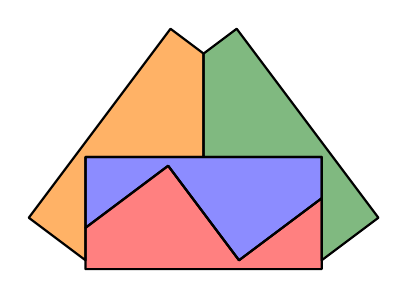
\begin{tikzpicture}[scale=1.5,line join=round,thick]
\fill[blue!45] (0,0)--(7/10,21/40)--(13/10,-11/40)--(2,1/4)--(2,3/5)--(0,3/5)--cycle;
\fill[orange!60] (0,-11/40)--(0,3/5)--(1,3/5)--(1,59/40)--(18/25,337/200)--(-12/25,17/200)--cycle;
\fill[green!45!black!50] (62/25,17/200)--(32/25,337/200)--(1,59/40)--(1,3/5)--(2,3/5)--(2,-11/40)--cycle;
\fill[red!50] (2,1/4)--(13/10,-11/40)--(7/10,21/40)--(0,0)--(0,-7/20)--(2,-7/20)--cycle;
\draw (0,0)--(7/10,21/40)--(13/10,-11/40)--(2,1/4)--(2,3/5)--(0,3/5)--cycle;
\draw (0,-11/40)--(0,3/5)--(1,3/5)--(1,59/40)--(18/25,337/200)--(-12/25,17/200)--cycle;
\draw (62/25,17/200)--(32/25,337/200)--(1,59/40)--(1,3/5)--(2,3/5)--(2,-11/40)--cycle;
\draw (2,1/4)--(13/10,-11/40)--(7/10,21/40)--(0,0)--(0,-7/20)--(2,-7/20)--cycle;
\end{tikzpicture}
\caption{A holeless tetrad of four congruent hexagons of the type found by
Scott Kim, with rational corner coordinates. The tile in the middle (blue)
touches each of the other three along a segment.}\label{fig:hex}
\end{figure}

\paragraph{History.} The Wikipedia article on the puzzle~\cite{wiki}
records, citing Gardner~\cite{gardner}, that the tetrad was named by
Michael R.~W. Buckley in 1975 in the \emph{Journal of Recreational
Mathematics}, that whether the four regions can be congruent, with or
without holes, became a puzzle, and that Scott Kim found a holeless
solution made of hexagons. \v{C}er\c{n}enoks and Cibulis~\cite[Section~6, Problem~P1]{cc}
write: ``In the book (Gardner, 1989) two full tetrads made of 6-gons are
given, and the question what the smallest $n$-gon is like has been
asked'' (a \emph{full} tetrad is a holeless one). Pentagons can form a
tetrad around a hole: Walter Trump~\cite{trump14} shows five such tetrads,
the oldest sent to Gardner in 1979 and one by Livio Zucca. On whether
pentagons can do without the hole, Trump writes~\cite{trump14}: ``It is
extremely unlikely that such a tetrad without hole exists, but I have not
seen a proof.'' His answer on hexagons is stated conditionally on ``the
conjecture that holeless pentagons cannot form a tetrad''~\cite{trump15}.
David Eppstein asked the same question in 2021 (``Is the hole
necessary?'')~\cite{eppstein}, and the Wikipedia article lists it as
unknown~\cite{wiki}. Trump also shows that convex tiles cannot form a
tetrad, even with holes~\cite{trump18}, and states that four quadrilaterals
cannot form a tetrad, asking for a short proof~\cite{trump13}.
Theorem~\ref{thm:main} proves Trump's conjecture, and
Corollary~\ref{cor:six} answers the question of the smallest $n$ for
holeless tetrads of congruent polygons. For quadrilaterals our argument
covers only holeless tetrads, so it does not settle Trump's statement about
quadrilaterals in general.

\paragraph{What is new.} The convex case is settled by Trump's
argument~\cite{trump18}. Without convexity a tile may have reflex
corners, a corner of one tile may lie inside a side of another, and two
tiles may meet along several segments. The first step of our proof bounds how
the tiles fit together, by Euler's formula. The resistant step is the last one: in
the 116 families of angle and length data that satisfy every linear
condition, the difficulty lies at degenerate points on the boundary of the
parameter region, where many of the relevant trigonometric polynomials
vanish at once, some to high order. Interval arithmetic alone cannot give
a strict sign on a cell containing such a point; we use exact
higher-order Taylor bounds and resultants there.

The proof depends on a computation, described in
Section~\ref{sec:verification}; the reduction to that computation
(Sections~\ref{sec:maps} and~\ref{sec:conditions}) is a written argument.

\section{Proof overview}

Fix a holeless tetrad of four congruent polygons with $n$ sides, copies of
a prototile $P$. The union of the tile boundaries is a connected plane graph
whose faces are the four tile interiors and one outer face. After removing
vertices of degree two, Euler's formula leaves a plane map with at most six
vertices and nine edges in which every two tiles share an edge. There are
exactly three such maps (Lemma~\ref{lem:maps}). For each map we enumerate
how the corners of each tile sit on it and which corner of $P$ each one is.
The angles of $P$ must then satisfy linear equations (the angles at a
vertex sum to $360^\circ$) and strict inequalities, and the side lengths
must satisfy linear equations (a side of one tile is covered by segments
shared with others). Deciding these systems exactly leaves, for $n=5$,
116 cases and none for $n=3,4$ (Lemma~\ref{lem:linear}).

In each surviving case the angles form a two-parameter family, an open
polygon $R$ in the plane of two free angles $(p,q)$, and the admissible side
lengths form the relative interior of a polyhedral cone with at most three
generators. The remaining condition is that $P$ closes up, a pair of
trigonometric equations, and is simple. Relabeling $P$ maps the 116 cases
onto one another in 22 classes. For one case in each class a certificate
subdivides $R$ into cells and shows on each cell, by exact and interval
arithmetic, that no admissible lengths close $P$ into a simple pentagon
(Lemma~\ref{lem:closure}).

\section{The boundary map}\label{sec:maps}

Let $T_1,\dots,T_4$ be the tiles of a holeless tetrad of congruent polygons
with $n$ sides, and let $N$ be the set of all corners of all tiles. Cut every
side of every tile at the points of $N$ on it; the resulting segments are
the \emph{pieces}.

\begin{lemma}\label{lem:graph}
Two pieces of different tiles are either equal or meet only at common
endpoints. The pieces form a connected plane graph $G$ with vertex set $N$,
whose faces are the four tile interiors and one outer face. At each vertex
$x$ of $G$, each tile containing $x$ occupies exactly one of the sectors
cut out by the edges at $x$, with angle equal to its corner angle at $x$ or
to $180^\circ$; the sector angles at $x$ sum to $360^\circ$, and at most one
tile sector at a vertex of degree at least three has angle $180^\circ$.
\end{lemma}

\begin{proof}
Let $s$ and $t$ be pieces of $T_i$ and $T_j$, $i\ne j$, sharing a point $x$
that is not an endpoint of both. If they are collinear and overlap, both are
maximal segments between consecutive points of $N$ on a common line, so
they coincide. If $x$ is interior to both and they cross, then near $x$ the
interior of $T_i$ is an open half-disk on one side of $s$, while the interior
of $T_j$ has points on both sides of $s$ near $x$; the interiors would meet.
If $x$ is an endpoint of $t$ and interior to $s$, then $x\in N$ and $s$ would
have been cut at $x$. So $G$ is a plane graph. It is connected because each
tile boundary is connected and every two boundaries meet.

The interior of each $T_i$ is connected and open, misses every other
boundary (a point of it on $\partial T_j$ would have interior points of
$T_j$ nearby), and has its frontier in $G$; so it is a face. Every other
point off $G$ lies outside the union $U$ of the tiles, so the remaining faces
are the components of $\R^2\setminus U$: one, since the tetrad is
holeless. Near a vertex $x$ on $\partial T_i$, the tile $T_i$ is a single
closed angular sector, and no edge of $G$ enters its interior; so it is one
sector of $G$ at $x$, of angle equal to its corner angle or $180^\circ$. Two
straight tile sectors would fill $360^\circ$ and leave only two sectors.
\end{proof}

A vertex of $G$ of degree two is a corner of some tile; we call it a
\emph{bend}. Its two sectors are not both outer, since every piece has a
tile on one side. If both are tile sectors, the bend is \emph{interior}:
the two angles sum to $360^\circ$ and neither is $180^\circ$, so it is a
corner of both tiles. If one sector is outer, the bend is
\emph{exterior}: it is a corner of the other tile, and the outer sector
has positive angle.

Suppress every bend, interior or exterior. The result is a connected plane
multigraph $M$ with the same five faces and all degrees at least three.
Each edge of $M$ carries the bends suppressed on it: interior bends on an
edge between two tiles, exterior bends on an edge between a tile and the
outer face.
Each edge of $M$ has two different faces on its sides, at least one a tile;
each tile boundary is a closed walk through each vertex at most once; and
every two tiles share an edge, since a common boundary segment of positive
length contains an interior point of a common piece. With $V$, $E$ and
$F=5$ the numbers of vertices, edges and faces, Euler's formula gives
$\sum_v(\deg v-2)=2E-2V=2(F-2)=6$, so $V\le 6$ and $E\le 9$.

\begin{lemma}\label{lem:maps}
Up to homeomorphism of the plane, $M$ is one of three maps:
\begin{itemize}
\item[(W)] one tile is surrounded by the other three, each of which meets
the outer face along an edge;
\item[(R)] two tiles meet the outer face and share two edges, enclosing the
other two tiles between them;
\item[(R$_0$)] as (R), except that one of the two shared edges shrinks to a
vertex at which one enclosed tile touches the outer face.
\end{itemize}
\end{lemma}

\begin{proof}
This is a finite enumeration. The plane dual $D$ of $M$ has the five faces
as vertices; it is connected, loopless and plane; every two tile vertices
are adjacent; and every face of
$D$ (a vertex of $M$) has length at least three and contains each tile at
most once. Enumerating all rotation systems on at most nine edges
satisfying these conditions gives exactly three maps up to isomorphism,
including mirror images. A separate enumeration of the primal maps $M$
directly, with $V\le6$ vertices of degree at least three and the
conditions above, gives the same three, with degree sequences
$3,3,3,3,4$ for (R$_0$) and $3,3,3,3,3,3$ for (R) and (W).
\end{proof}

\section{Angle and length conditions}\label{sec:conditions}

Let $a_0,\dots,a_{n-1}$ be the angles of $P$ and $\ell_0,\dots,\ell_{n-1}$ its
side lengths, side $i$ joining corners $i$ and $i+1$ in counterclockwise
order (indices mod $n$). A \emph{placement} records, for each tile, which of
its sectors at vertices of $M$ are corners and which are straight, and how
many bends lie on each edge of $M$, so that each tile has $n$ corners; an
interior bend counts as a corner of both its tiles, and an exterior bend as
a corner of its one tile. A
\emph{labeling} identifies the corners of each tile with those of $P$: if
the tile is a direct copy of $P$, corner $k$ of the tile is corner $s+k$ of
$P$ and the side after it is side $s+k$; if the tile is a mirror copy,
corner $k$ is corner $s-k$ and the side after it is side $s-k-1$. Applying
an isometry to the whole tetrad, we may take the tile on a fixed face of
the representative map to be $P$ itself, so the labelings of the other
three tiles range over the $2n$ identifications each. Finally a
\emph{reflex pattern} says which $a_i$ exceed $180^\circ$.

Each tetrad yields a map, a placement, a labeling and a reflex pattern for
which the following hold:
\begin{itemize}
\item \emph{angles}: $\sum_i a_i=(n-2)\cdot180^\circ$; the tile sectors at a
vertex of $M$ sum to $360^\circ$ when no sector is outer and to less than
$360^\circ$ otherwise; the two corners at an interior bend sum to
$360^\circ$, while an exterior bend imposes no equation; each $a_i$ lies in
$(0^\circ,180^\circ)$ or $(180^\circ,360^\circ)$ as the pattern says;
\item \emph{lengths}: on an edge of $M$ with $b$ bends, interior or
exterior, there are $b+1$ segments of positive length, one between each
two consecutive vertices of $G$ on it; each side of each tile is a run of such
segments through vertices where the tile is straight, and its length is
the sum of theirs and equals $\ell_i$ for its label $i$.
\end{itemize}
Both systems are linear, with strict inequalities, and share no
variables.

\begin{lemma}\label{lem:linear}
For $n=3$ and $n=4$ no map, placement, labeling and pattern has a feasible
angle system. For $n=5$ there are $54{,}938$ placements; exactly $2{,}850$
of their labeled, patterned versions have a feasible angle system, and
exactly $116$ of these also have a feasible length system.
\end{lemma}

\begin{proof}
A depth-first search assigns labelings tile by tile, pruning by interval
bounds on the angles, and decides each complete system by linear
programming in exact rational arithmetic: it maximizes a common slack $t$
in all strict inequalities and accepts if and only if the optimum is
positive. Appendix~\ref{app:counts} lists the counts by map. A separate
implementation, written from a specification of the conditions without
access to the search and using exact polyhedra, reproduces every count by map
for $n=3,4,5$.
\end{proof}

For each of the 116 cases the angle equalities have rank $n-2=3$, so the
angles form a two-parameter family $a_i=A_ip+B_iq+C_i$ with integers
$A_i,B_i,C_i$ and two free angles $p,q$; the strict inequalities cut out an
open convex polygon $R$ in the $(p,q)$-plane. The admissible length vectors
$\ell$ are the relative interior of the projection $L$ of the cone of
nonnegative solutions of the length equalities, since a strictly positive
solution exists. In every case $L$ is generated by $m\le3$ integer rays
$r_1,\dots,r_m$, so the admissible $\ell$ are the sums $\sum_j\mu_jr_j$ with
all $\mu_j>0$.

\section{Closure and simplicity}\label{sec:closure}

Let $\theta_0=0$ and $\theta_{i+1}=\theta_i+180^\circ-a_{i+1}$ be the
directions of the sides of $P$, and $u_i=\cos\theta_i+\sqrt{-1}\sin\theta_i$. The prototile closes
up if and only if $\sum_i\ell_iu_i=0$, that is, $\sum_j\mu_jv_j=0$ with
$v_j=\sum_i r_{j,i}u_i$. It is simple if and only if no two non-adjacent
sides meet. With $Z=\cos\frac p2+\sqrt{-1}\sin\frac p2$ and $W=\cos\frac q2+\sqrt{-1}\sin\frac q2$, each
$u_i$ is $\pm Z^{2s}W^{2t}$, where $s$ and $t$ are the integer coefficients
of $p$ and $q$ in $\theta_i$, so every quantity in these conditions is a
Laurent polynomial in $Z$ and $W$ restricted to the torus $|Z|=|W|=1$.

Closure with all $\mu_j>0$ splits into branches. For $m=1$ it needs
$v_1=0$. For $m=2$ there are two branches: the degenerate one, $v_1=v_2=0$,
on which every $\mu>0$ closes $P$; and the generic one, $v_1$ and $v_2$
nonzero with $v_1\times v_2=0$ and $v_1\cdot v_2<0$, on which
$\mu=(-v_1\cdot v_2,\,|v_1|^2)$ up to a positive factor. For $m=3$ write
$c_{12}=v_1\times v_2$, $c_{23}=v_2\times v_3$ and $c_{31}=v_3\times v_1$.
On the generic branch the three are all positive or all negative, and
$\mu=\sigma(c_{23},c_{31},c_{12})$ up to a positive factor, $\sigma$ being
their common sign. On the degenerate branch all three vanish, so
$v_1,v_2,v_3$ are collinear and $\mu$ is not determined. Only on the
generic branches (and for $m=1$, where $\mu$ is a single positive number)
is $\mu$ substituted into the conditions that sides $i$ and $j$ meet, which
then become sign conditions on finitely many trigonometric polynomials in
$p,q$. A degenerate branch is excluded from necessary conditions alone,
without choosing $\mu$: it requires two of the closure quantities
($|v_1|^2$ and $|v_2|^2$ for $m=2$; two of the cross products for $m=3$)
to vanish at a common point.

\begin{lemma}\label{lem:closure}
For each of the 116 cases, no $(p,q)\in R$ and $\mu>0$ make $P$ a closed
simple pentagon.
\end{lemma}

\begin{proof}
Relabeling the corners of $P$ (rotating or reflecting its labels) maps
cases to cases and preserves closure and simplicity. Under it the 116
cases fall into 22 classes, and for every case an explicit relabeling onto
a chosen member of its class is checked to carry its angle family, region
and length cone exactly onto that member's. It is enough to treat the
chosen members.

For 21 classes the chosen member has a certificate. It lists, for every
closure and simplicity quantity $Q$, an identity $Q=K\prod_kg_k^{e_k}$ on the
torus with $K$ a nonzero real constant and each $g_k$ a real Laurent
polynomial with Gaussian rational coefficients or a product $ff^*=|f|^2$;
and a subdivision of a box containing $R$ into cells, each with a reason why
no sign pattern of the factors that is possible on the cell satisfies the
closure branch and simplicity. Appendix~\ref{app:signs} lists the sign rules, including
how degenerate closure branches are excluded.

The remaining class has $m=1$ and is closed by an identity. Its angles are
$a=(180-p-q,\,180+q,\,180-q,\,p,\,q)$ with $0<p+q<180$, and its ray is
$r=(1,2,1,2,1)$. A direct computation gives
\[
\operatorname{Re}\bigl(ZW\,v_1\bigr)=3\cos\frac{\pi(p+q)}{360},
\]
which is positive on $R$, so $v_1\ne0$ and $P$ cannot close.
\end{proof}

\begin{proof}[Proof of Theorem~\ref{thm:main} and Corollary~\ref{cor:six}]
A holeless tetrad of four congruent polygons with $n$ sides gives, by
Lemmas~\ref{lem:graph} and~\ref{lem:maps} and Section~\ref{sec:conditions},
one of the enumerated maps, placements, labelings and patterns, with angles
and lengths satisfying the linear systems, and with $P$ closed and simple.
For $n=3,4$ Lemma~\ref{lem:linear} leaves no case. For $n=5$ it leaves the
116 cases, and Lemma~\ref{lem:closure} excludes each. With Kim's hexagonal
tetrad (Figure~\ref{fig:hex}), six is the least number of sides.
\end{proof}

\section{Computational verification}\label{sec:verification}

The computer checks Lemmas~\ref{lem:maps}, \ref{lem:linear}
and~\ref{lem:closure} and the relabeling reduction; Lemma~\ref{lem:graph}
and the translation into placements and linear systems are the written
argument above. The certificates are checked by a verifier written
separately from the programs that produced them, from a specification of
the conditions alone, with its own interval arithmetic (outward-rounded
intervals of the \texttt{mpmath} library rather than the ball arithmetic
used to produce them). It rederives each case's angle family, region and
length cone, checks every factorization identity symbolically, replays the
subdivision, and rejects corrupted certificates. The identity for the remaining
class is checked by two separate symbolic computations.

With the accompanying code and data, checking the map enumerations, the
cover and every certificate takes about three minutes on two cores;
rerunning the exact angle screen takes about
five CPU-hours. Appendix~\ref{app:signs} also describes tests of the reduction.

\begin{appendices}
\section{Counts}\label{app:counts}

\begin{table}[h]
\centering
\begin{tabular}{lrrr}
\toprule
& (R$_0$) & (R) & (W)\\
\midrule
placements, $n=3$ & 284 & 190 & 722\\
placements, $n=4$ & 1{,}986 & 2{,}250 & 7{,}698\\
placements, $n=5$ & 7{,}078 & 12{,}040 & 35{,}820\\
angle-feasible, $n=5$ & 60 & 36 & 2{,}754\\
also length-feasible, $n=5$ & 4 & 4 & 108\\
\bottomrule
\end{tabular}
\caption{Placements and feasible labeled cases by map. For $n=3,4$ no case
is angle-feasible. The 116 length-feasible cases form 22 classes under
relabeling of $P$: four of size two and eighteen of size six.}
\end{table}

\section{Sign rules and tests}\label{app:signs}

The certificates of Lemma~\ref{lem:closure} decide signs on a cell as
follows. The sign of a factor $\rho\cos(k_pp+k_qq+\delta)$
on a cell follows from the exact range of its phase; other factors are
bounded by interval arithmetic. Near a point $c$ where several factors
vanish (a vertex of $R$ or a point inside it), the certificate uses polar
cells around $c$ and the exact
order $k$ of vanishing of each factor at $c$ (all partial derivatives of
order below $k$ vanish, tested in the cyclotomic field) together with the
Taylor remainder of order $k+1$. On a degenerate closure branch, and
wherever else two factors would have to vanish at a common point of a
cell, either one of them has a strict sign on the cell or the resultants in
$W$ and in $Z$ show that they have no common zero there.

As a test of the reduction, the same programs applied to
hexagons find holeless tetrads of congruent hexagons, one of Kim's type,
without being given an example; and drawings of Kim's tetrad and of
several pentagon tetrads with a hole are found by the placement and
labeling search with their actual labeling.
\end{appendices}

\begin{thebibliography}{9}
\bibitem{cc} J.~\v{C}er\c{n}enoks and A.~Cibulis, Tetrads and their
counting, \emph{Baltic J. Modern Computing} \textbf{6} (2018), no.~2,
96--106, \url{https://doi.org/10.22364/bjmc.2018.6.2.01}.

\bibitem{eppstein} D.~Eppstein, Linkage, blog post, April 30, 2021,
\url{https://11011110.github.io/blog/2021/04/30/linkage.html}.

\bibitem{gardner} M.~Gardner, \emph{Penrose Tiles to Trapdoor Ciphers},
W.~H. Freeman, 1989, pp.~121--123.

\bibitem{trump13} W.~Trump, Further questions about tetrads, Question~13:
Can four quadrilaterals form a tetrad?, February 12, 2020,
\url{https://www.trump.de/tetrads/question-13/question-13.htm}.

\bibitem{trump14} W.~Trump, Further questions about tetrads, Question~14:
Can four pentagons form a tetrad?, February 12, 2020,
\url{https://www.trump.de/tetrads/question-14/question-14.htm}.

\bibitem{trump15} W.~Trump, Further questions about tetrads, Question~15:
Which tetrads can be made with hexagons?, February 12, 2020,
\url{https://www.trump.de/tetrads/question-15/question-15.htm}.

\bibitem{trump18} W.~Trump, Further questions about tetrads, Question~18:
Are convex tiles possible?, February 19, 2020, last modified April 2, 2025,
\url{https://www.trump.de/tetrads/question-18/question-18.htm}.

\bibitem{wiki} Wikipedia, Tetrad (geometry puzzle), revision of June 16,
2026,
\url{https://en.wikipedia.org/w/index.php?title=Tetrad_(geometry_puzzle)&oldid=1359635574}.
\end{thebibliography}
\end{document}
